\documentclass[12pt]{article}
\usepackage[left=0.5in, right=0.5in, top=0.5in, bottom=0.5in]{geometry}
\usepackage{ulem}
\usepackage{amsmath}
\usepackage{amssymb}
\usepackage{enumerate}
\usepackage{tikz}
\def\checkmark{\tikz\fill[scale=0.4](0,.35) -- (.25,0) -- (1,.7) -- (.25,.15) -- cycle;}
\usepackage{graphicx}
\graphicspath{ {images/} }

\begin{document}
\begin{flushleft}
Andy Liang

CSE 150 - Foundations of Computer Science: Honors

Professor Bender
\end{flushleft}
\medskip
\centerline{\uline{Homework 3A}}
\bigskip\bigskip



\noindent
\uline{Problem 2}
\\*\textbf{Show that every subset of $\mathbb{N}$ is countable.}
\bigskip
\\*\uline{Proof}
\bigskip
\\* Let X$_n$ be a subset of $\mathbb{N}$ with $n$ elements. We show that X$_n$ is countable by showing that the cardinality of X$_n$ is either equal to or less than the cardinality of $\mathbb{N}$, which is, by definition, a countably infinite set.
\bigskip
\\* Let $f$ : X$_n$ $\rightarrow \mathbb{N}$.  Set $f(X_n) = n$. We show that $f$ can have a cardinality equal to $\mathbb{N}$ by showing that there is a bijection between X$_n$ and $\mathbb{N}$.
\bigskip
\\* First observe that $f$ is one-to-one. This is true because if $f(a) = f(b)$ for some a, b $\in$ X$_n$, then a = b.
\bigskip
\\* Now we show that $f$ is onto for some $n$. If $n = \infty$, then the cardinality of $X_n$ is equal to the cardinality of $\mathbb{N}$ so for all $a \in {N}$ there exists $b \in X_n$ such that $f(b) = a$.
\bigskip
\\* Now we show that $f$ is not onto for some $n$. If $n < \infty$, then the cardinality of $X_n$ is less than the cardinality of $\mathbb{N}$ so there exists $b \in {X_n}$ such that there exists no $a \in $ that satisfies $f(b) = a$. 
\bigskip
\\* Thus, $f$ is a bijection or an injection and $X_n$ is countable. 
\bigskip



\noindent
\uline{Problem 3}
\\*\textbf{Show that the set of all integers ($\mathbb{Z}$) is countable.}
\bigskip
\\*\uline{Proof}
\\* We show that $\mathbb{Z}$ is countable by showing a bijection between $\mathbb{Z}$ and $\mathbb{N}$.
\bigskip
\\*Let f: $\mathbb{N} \rightarrow \mathbb{Z}$.
Set $f(x) =$ \[ \begin{cases}
			x/2$, if x is even$ \\
			-(x+1)/2$, if x is odd$ \\
		\end{cases}
		\]
\\* $\mathbb{N} = \{0, 1, 2, 3, 4, ,...\}$
\\* $\mathbb{Z} = \{0, -1, 1, -2, 2, ...\}$
\\* First observe that $f$ is one-to-one. This is true because if $f(a) = f(b)$ for some $a,b \in X$, then $a/2 = a/b$ if $a$ and $b$ are even and $-(a+1)/2 = -(b+1)/2$ if $a$ and $b$ are odd, both implying that $a = b$.
\bigskip
\\* Now we show that $f$ is onto. We need to show that for all $a \in \mathbb{Z}$, there exists $b$ such that $f(b) = a$ and $b$ is in $\mathbb{N}$. 
\\*Assume $b$ is positive. Let $b = 2a$. Then $f(b) = f(2a) = 2a/2 = a$. 
\\*Assume $b$ is negative. Let $b = -(2a + 1)$. Then $f(-(2a + 1)) = -(-(2a + 1) + 1)/2 = a$. 
\\*Since $a \in \mathbb{Z}$, it can be either positive or negative. When $a$ is positive, $2a$ is also positive. When $a$ is negative, $-(2a + 1)$ is positive. Therefore, $b = 2a$ when a is positive and $b = -(2a + 1)$ when a is negative are both in $\mathbb{N}$.
\bigskip
\\*Thus, $f$ is a bijection and $\mathbb{Z}$ is countable. 
\bigskip



\noindent
\\*\uline{Problem 4}
\\*\textbf{Show that the set of all \textit{finite} subsets of a countable set is countable.}
\smallskip
\\*\uline{Proof}
\\* Let F be the set of all finite subsets of a countable set 
\\* We show that F is countable by showing a bijection between S and $\mathbb{N}$.
\bigskip
\\* A finite subset of a countable set can be represented as:
\\* $S_n, k$, where $n$ equals the $n$th subset of the countable set and $k$ represents the $k$th of elements of $S_n$ , = $\{S_{n,1}, S_{n,2}, S_{n,3},...,S_{n, k-1}, S_{n, k}\}$. 
\\* Then F can be represented as the set of all the finite sets: $\{S_1, S_2, S_3, ...\}$ which can be mapped bijectively to $\mathbb{N}$ and therefore is countable.
\medskip



\noindent
\\*\uline{Problem 5}
\\*\textbf{Show that the following statements are equivalent and true (Statement P and Q are \textit{equivalent} if P $\iff$ Q):}
\begin{itemize}
\item \textbf{$\mathbb{N}$ x $\mathbb{N}$ is countable.}
\bigskip
\\*\uline{Proof}
\\* Let $S$ be the set of $\mathbb{N} x \mathbb{N}$.
\\*We will prove that $S$ is countable by showing there is a bijection between $S$ and $\mathbb{N}$.
\bigskip
\\* Let f: $S \rightarrow \mathbb{N}$. Set $f(S_a) = \mathbb{N}_a$. 
\bigskip
\\* First observe that $f$ is one-to-one by definition of a function.
\bigskip
\\*Now we show that $f$ is onto. We need to show that for all $a \in \mathbb{N}$, there exists $b \in S$ such that $f(\mathbb{N}_a) = S_n$. We can do this by organizing the set of S as follows:
\\*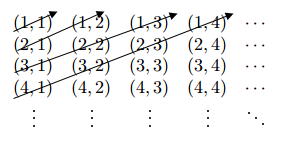
\includegraphics {NxN} %http-//i.stack.imgur.com/0s5hd
\\* where S = $\{n_{(1,1)}, n_{(2,1)}, n_{(2,2)}, n_{(3,1)},...\}$
\\* $\mathbb{N}$ = \{1, 2, 3, 4,...\} and can be mapped onto every element of S so f is also onto.
\bigskip
\\* Thus, $f$ is a bijection and $\mathbb{N}$ x $\mathbb{N}$ is countable.
\bigskip
\newpage




\item \textbf{Union of countably many countable sets is countable.}
\bigskip
\\*\uline{Proof}
\bigskip
\\* We will prove that the union of countably many countable sets is countable by using diagonalization.
\medskip
\\* The problem establishes that the sets are countable meaning they can be represented as:
\\* $S_n$, which represents the $n$th set, = $\{S_{n, 1}, S_{n, 2}, S_{n, 3},...\}$.
\\* We can then represent the elements of all the sets as:
\\*\begin{tabular}{cccccc}
\\* $S_{1,1}$ & $S_{1, 2}$ & $S_{1,3}$ & $S_{1,4}$ & $S_{1,5}$ & ... \\
\\* $S_{2,1}$ & $S_{2, 2}$ & $S_{2,3}$ & $S_{2,4}$ & $S_{2,5}$ & ... \\
\\* $S_{3,1}$ & $S_{3, 2}$ & $S_{3,3}$ & $S_{3,4}$ & $S_{3,5}$ & ... \\
\\* $S_{4,1}$ & $S_{4, 2}$ & $S_{4,3}$ & $S_{4,4}$ & $S_{4,5}$ & ... \\
\\* $S_{5,1}$ & $S_{5, 2}$ & $S_{5,3}$ & $S_{5,4}$ & $S_{5,5}$ & ... \\
\\*  ... & ... & ... & ... & ... & ...\\
\end{tabular}
\bigskip
\\*The set of the union of countably any countable sets can be represented as:
\\*$\{S_{1,1}, S_{2,1}, S_{2,2}, S_{3,1},...\}$
\\* which can be mapped bijectively to $\mathbb{N}$ and therefore is countable.
\bigskip



\item \textbf{$\mathbb{Q}$ is countable. }
\bigskip
\\*\uline{Proof}
\bigskip
\\* We will prove that $\mathbb{Q}$ is countable by showing there is a bijection between $\mathbb{Q}$ and $\mathbb{N}$ through diagonalization.
\bigskip
\\* The $\mathbb{Q}$ is the set of all numbers p/q, where p and q are both integers, so we can represent the set of $\mathbb{Q}$ as:
\\*\begin{tabular}{c|cccc}
\\* & 1 & 2 & 3 & ... \\
\hline
\\* 1 & 1/1 & 2/1 & 3/1 & ...\\
\\* 2 & 1/2 & 2/2 & 3/2 & ...\\
\\* 3 & 1/3 & 2/3 & 3/3 & ...\\
\\* ... & ... & ... & ... & ... 
\end{tabular}
\bigskip
\\* The set of $\mathbb{Q}$ can be represented as:
\\* $\{ 1/1, 1/2, 2/1, 1/3, 2/2, 3/1,...\}$
\\* which can be mapped bijectively to $\mathbb{N}$ and therefore is countable.
\end{itemize}
\bigskip



\noindent
\uline{Problem 6}
\\*\textbf{A submarine is moving along the integer number line at a constant speed $s$ so that at each hour it is on an integer number. It started moving at time 0 at some position $b$. If $t$ is the (whole) number of hours elapsed since the submarine started moving, then its position is given by the equation $x = st + b$, where $x, s$, and $b$ are integers.}
\\*\\*\textbf{You are working at Rocket Pizza delivery and you are to deliver pizza to the submarine. At each hour you can drop pizza on any number on the integer line. If the submarine is there at that time, then you have delivered the pizza and your job is done (you will be notified as soon as it happens).}
\\*\\*\textbf{The problem is that you don't know where the submarine is, you cannot see it, you don't know where it started and how fast it is moving (i.e., you don't know values of $s$ and $b$ - classified top secret data). The upside is that you have infinite number of pizzas.}
\\*\\*\textbf{Show that you can deliver pizza in a finite amount of time.}
\smallskip
\\*\uline{Response}
\\* I do not know how to solve this problem.
\newpage
\noindent
\uline{Problem 7}
\\*\textbf{The goal of this quiz/question is to make sure you will have no problems with countability in the future.
\bigskip
In the following table, F stands for Finite, I for Infinitely Countable, C for Countable, U for uncountable. Put a checkmark next
to the strongest statement you can make about the resulting set (i.e. correct answer for $F \cup F$ is finite, even though it is 
countable as well). Check \textbf{?} whenever there's not enough information to decide, i.e. there can be different cases with 
no `strongest' answer.}

\bigskip
\noindent
\uline{Response}
\begin{center}
	\begin{tabular}{c|c|c|c|c|c|c|c|c|c|c|c|c} \hline
  Set & F & I & C & U & ? & $\star$ & Set & F & I & C & U & ?  \\ \hline

$F \cup F$ & \checkmark & & & & & $\star$ & $C \cup F$ & & & \checkmark & & \\ \hline
$F \cup I$ & & \checkmark & & & & $\star$ & $C \cup I$ & & \checkmark & & & \\ \hline
$F \cup C$ & & & \checkmark & & & $\star$ & $C \cup C$ & & & \checkmark & & \\ \hline
$F \cup U$ & & & & \checkmark & & $\star$ & $C \cup U$ & & & & \checkmark & \\ \hline
$F \cap F$ & \checkmark & & & & & $\star$ & $C \cap F$ & & & \checkmark & & \\ \hline
$F \cap I$ & \checkmark & & & & & $\star$ & $C \cap I$ & & & \checkmark & & \\ \hline
$F \cap C$ & \checkmark & & & & & $\star$ & $C \cap C$ & & & \checkmark & & \\ \hline
$F \cap U$ & \checkmark & & & & & $\star$ & $C \cap U$ & & & \checkmark & & \\ \hline
$F - F$ & \checkmark & & & & & $\star$ & $C - F$ & & & \checkmark & & \\ \hline
$F - I$ & \checkmark & & & & & $\star$ & $C - I$ & & & \checkmark & & \\ \hline
$F - C$ & \checkmark & & & & & $\star$ & $C - C$ & & & \checkmark & & \\ \hline
$F - U$ & \checkmark & & & & & $\star$ & $C - U$ & & & \checkmark & & \\ \hline
$F \times F$ & \checkmark & & & & & $\star$ & $C \times F$ & & & \checkmark & & \\ \hline
$F \times I$ & & \checkmark & & & & $\star$ & $C \times I$ & & & \checkmark & & \\ \hline
$F \times C$ & & & \checkmark & & & $\star$ & $C \times C$ & & & \checkmark & & \\ \hline
$F \times U$ & & & & \checkmark & & $\star$ & $C \times U$ & & & & \checkmark & \\ \hline
$I \cup F$ & & \checkmark & & & & $\star$ & $U \cup F$ & & & & \checkmark & \\ \hline
$I \cup I$ & & \checkmark & & & & $\star$ & $U \cup I$ & & & & \checkmark & \\ \hline
$I \cup C$ & & \checkmark & & & & $\star$ & $U \cup C$ & & & & \checkmark & \\ \hline
$I \cup U$ & & & & \checkmark & & $\star$ & $U \cup U$ & & & & \checkmark & \\ \hline
$I \cap F$ & \checkmark & & & & & $\star$ & $U \cap F$ & & & & & \checkmark \\ \hline
$I \cap I$ & & & \checkmark & & & $\star$ & $U \cap I$ & & & & & \checkmark \\ \hline
$I \cap C$ & & & & \checkmark & & $\star$ & $U \cap C$ & & & & & \checkmark \\ \hline
$I \cap U$ & & & & & \checkmark & $\star$ & $U \cap U$ & & & & \checkmark & \\ \hline
$I - F$ & & \checkmark & & & & $\star$ & $U - F$ & & & & \checkmark & \\ \hline
$I - I$ & & & \checkmark & & & $\star$ & $U - I$ & & & & \checkmark & \\ \hline
$I - C$ & & & \checkmark & & & $\star$ & $U - C$ & & & & \checkmark & \\ \hline
$I - U$ & & & \checkmark & & & $\star$ & $U - U$ & & & & \checkmark & \\ \hline
$I \times F$ & & \checkmark & & & & $\star$ & $U \times F$ & & & & \checkmark & \\ \hline
$I \times I$ & & \checkmark & & & & $\star$ & $U \times I$ & & & & \checkmark & \\ \hline
$I \times C$ & & \checkmark & & & & $\star$ & $U \times C$ & & & & \checkmark & \\ \hline
$I \times U$ & & & & \checkmark & & $\star$ & $U \times U$ & & & & \checkmark & \\ \hline
\end{tabular}
\end{center}

\end{document}